\documentclass[11pt,a4paper,onecolumn]{article}
\usepackage[left=3cm,right=3cm,top=2cm,bottom=2cm]{geometry}
\usepackage{amsmath}
\usepackage{float}
\usepackage{graphicx}
\DeclareGraphicsExtensions{.eps,.ps,.jpg,.bmp,.pdf}
\usepackage{ctex}
\usepackage{url}
\usepackage{listings}
\usepackage{color}
\definecolor{mygreen}{rgb}{0,0.6,0}
\definecolor{mygray}{rgb}{0.5,0.5,0.5}
\definecolor{mymauve}{rgb}{0.58,0,0.82}
\lstset{
	backgroundcolor=\color{white},
	basicstyle=\footnotesize,
	breakatwhitespace=false,
	breaklines=true,
	captionpos=b,
	commentstyle=\color{mygreen},
	deletekeywords={...},
	extendedchars=true,
	keepspaces=true,
	keywordstyle=\color{blue},
	language=R,
	otherkeywords={*,...},
	numbers=left,
	numbersep=5pt,
	numberstyle=\tiny\color{mygray},
	rulecolor=\color{black},
	showspaces=false,
	showstringspaces=false,
	showtabs=false,
	stepnumber=1,
	stringstyle=\color{mymauve},
	tabsize=2,
	}

\begin{document}
\title{\bfseries 使用R实现分类树算法}
\date{}
\author{黎思言}
\maketitle

\section{表二数据。以Entropy为计算不纯度标准,构建二叉树的第一层划分。}

(1)第一步:计算未分类之前的熵

\begin{align*}
	I_0 &=-\sum_{i=1}^kp(i|0)log_2p(i|0) \\
      &=-(\frac{3}{10}*log_2(\frac{3}{10})+\frac{7}{10}*log_2(\frac{7}{10})) \\
			&=0.88
\end{align*}

(2)第二步:计算不同分类标准下的熵

如果按照日志密度进行分组,会有三种情况(将s分到一组,m和l分到另一组;将m分到一组,s和l分到另一组;将l分到一组,s和m分到另一组),这三种情况下的熵分别是:

\begin{align*}
	I_{11} &=-(\frac{3}{10}(\frac{1}{3}*log_2(\frac{1}{3})+\frac{2}{3}*log_2(\frac{2}{3})) \\
			&\quad+ \frac{7}{10}(\frac{6}{7}*log_2(\frac{6}{7})+\frac{1}{7}*log_2(\frac{1}{7}))) \\
			&=0.69
\end{align*}

\begin{align*}
	I_{12} &=-(\frac{4}{10}(\frac{3}{4}*log_2(\frac{3}{4})+\frac{1}{4}*log_2(\frac{1}{4}) )\\
			&\quad+ \frac{6}{10}(\frac{2}{6}*log_2(\frac{2}{6})+\frac{4}{6}*log_2(\frac{4}{6}))) \\
			&=0.88
\end{align*}

\begin{align*}
	I_{13} &=-(\frac{3}{10}(\frac{0}{3}*log_2(\frac{0}{3})+\frac{3}{3}*log_2(\frac{3}{3})) \\
			&\quad+ \frac{7}{10}(\frac{3}{7}*log_2(\frac{3}{7})+\frac{4}{7}*log_2(\frac{4}{7}))) \\
			&=0.69
\end{align*}

如果按照好友密度进行分组,将有三种情况(将s分到一组,m和l分到另一组;将m分到一组,s和l分到另一组;将l分到一组,s和m分到另一组),这三种情况下的熵分别是:

\begin{align*}
	I_{21} &=-(\frac{4}{10}(\frac{3}{4}*log_2(\frac{3}{4})+\frac{1}{4}*log_2(\frac{1}{4})) \\
			&\quad+ \frac{6}{10}(\frac{0}{6}*log_2(\frac{0}{6})+\frac{6}{6}*log_2(\frac{6}{6}))) \\
			&=0.32
\end{align*}

\begin{align*}
	I_{22} &=-(\frac{4}{10}(\frac{0}{4}*log_2(\frac{0}{4})+\frac{4}{4}*log_2(\frac{4}{4})) \\
			&\quad+ \frac{6}{10}(\frac{3}{6}*log_2(\frac{3}{6})+\frac{3}{6}*log_2(\frac{3}{6}))) \\
			&=0.6
\end{align*}

\begin{align*}
	I_{23} &=-(\frac{2}{10}(\frac{0}{2}*log_2(\frac{0}{2})+\frac{2}{2}*log_2(\frac{2}{2})) \\
			&\quad+ \frac{8}{10}(\frac{3}{8}*log_2(\frac{3}{8})+\frac{3}{8}*log_2(\frac{3}{8}))) \\
			&=0.76
\end{align*}

如果按照是否使用真实头像分组,将有一种情况(将yes分到一组,no分到另一组),这种情况下的熵是:

\begin{align*}
	I_3 &= -(\frac{5}{10}(\frac{2}{5}*log_2(\frac{2}{5})+\frac{2}{5}*log_2(\frac{2}{5})) \\
			&\quad+ \frac{5}{10}(\frac{4}{5}*log_2(\frac{4}{5})+\frac{1}{5}*log_2(\frac{1}{5}))) \\
			&=0.85
\end{align*}

(3)第三步:计算熵的变化

对于以上7种分类标准,分别计算出熵的变化。

\begin{align*}
	I_0-I_{11} &=0.19 \\
	I_0-I_{12} &=0.005 \\
	I_0-I_{13} &=0.19 \\
	I_0-I_{21} &=0.56 \\
	I_0-I_{22} &=0.28 \\
	I_0-I_{23} &=0.12 \\
	I_0-I_3 &=0.03 \\
\end{align*}

(4)第五步:选取分类标准

对于以上计算出的7个熵的变化值,取熵减少量最大的分类标准作为第一次分类的分类标准。所以,选择好友密度为分类标准,将好友密度小归为一类,将好友密度中和好友密度大归为另一类。

\section{第二题:表一Quinlan(1986)数据。用R中的rpart包建立决策树,注意决策树的控制条件的设定并对表三数据进行预测。}

第一步:加载rpart包。第二步:读入数据。第三步:建立分类树模型,注意将参数调整为叶节点上至少有一个数据。第四步:用模型预测表3的数据。第五步:查看结果。

代码:

\begin{lstlisting}
	library(rpart)
	biao1=read.csv("表1.csv",header = T)
	biao3=read.csv("表3.csv",header = T)
	mod=rpart(PLAY~.,data=biao1,method="class",
          control=rpart.control(minbucket=1,cp=0.01))
	biao3
  play_hat=predict(mod,newdata=biao3)
  play_hat
\end{lstlisting}

结果:

\begin{lstlisting}
	> play_hat
    Don't play play
  1          0    1
  2          0    1
\end{lstlisting}

结果显示,我们的CART分类器将表3中的两个样本都归类到play类了。

\section{第三题:iris数据。用R中的rpart包,用二折交叉验证估计CART的误差。}

第一步:加载iris数据。第二步:写一个交叉验证函数(详情见注释)。第三步:通过二折交叉验证计计算在不同的minbucket下模型的准确率。第四步:挑选准确率最高的模型。

代码:

\begin{lstlisting}	mycv=function(formula=Species~.,data=iris,minbucket=c(1:20),k=2){
		#minbucket=c(1:20),表示待定参数从c(1:20)中产生,k=2表示进行二折交叉验证。
		n=nrow(data)
		m=n%/%k
		data=data[sample(1:n,n),] #shuffle数据
		result=matrix(NA,nrow=length(minbucket),ncol=k)
		for(i in 1:length(minbucket)){
			for(j in 1:k){
				index=c(((j-1)*m+1):(j*m))
				valid=data[index,] #验证集
				train=data[-index,] #训练集
				mod=rpart(formula,data=train,method="class",
									control=rpart.control(minbucket=minbucket[i]))
				y_hat=predict(mod,newdata = valid)
				y_hat=apply(y_hat,1,function(x)names(which.max(x)))
				acc=sum(y_hat==valid$Species)/m #计算准确率
				result[i,j]=acc
				}
			}
		result=rowMeans(result)
		return(list(minbucket=minbucket,acc=result))
		}

		set.seed(100)
		cv=mycv()
		png("交叉验证.png",width = 700,height = 500)
		ggplot(data=data.frame(minbucket=cv$minbucket,Accuracy=cv$acc),aes(x=minbucket,y=Accuracy))+
		geom_point(size=5,shape=15)+
		geom_line(size=1)+
		theme_bw()+
		theme(axis.title = element_text(size=20),
					axis.text = element_text(size=15))
		dev.off()
\end{lstlisting}

结果:

\begin{figure}[H]
	\centering
	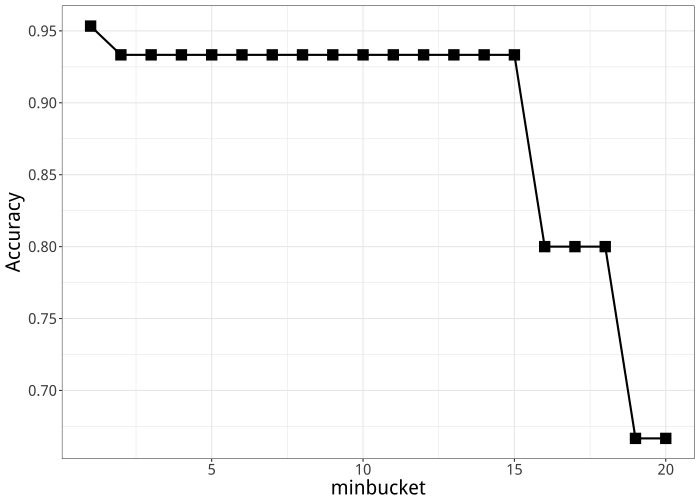
\includegraphics[width=300pt]{交叉验证.png}
	\caption{二折交叉验证的准确率}
\end{figure}

从图1可知,二折交叉验证显示,当minbucket取1的时候,CART分类器的准确率是最高的。所以我用我使用四分之三的数据做训练集,用四分之一的数据做测试集,使用minbucket=1重新构建了模型,代码和预测结果如下。

\begin{lstlisting}
set.seed(100)
data=iris[sample(1:nrow(iris),nrow(iris)),]
train=sample(1:nrow(iris),nrow(iris)%/%4*3)
mod=rpart(Species~.,data=data,method="class",subset = train,
          control=rpart.control(minbucket=1))
y_hat=predict(mod,newdata = data[-train,])
y_hat=apply(y_hat,1,function(x)names(which.max(x)))
sum(y_hat==data$Species[-train])/length(data$Species[-train])
table(y_hat,data$Species[-train])
\end{lstlisting}

\begin{table}[H]
\centering
\caption{预测结果}
\begin{tabular}{cccc}
  \hline
              & setosa & versicolor & virginica \\
  setosa      & 11     & 0          & 0         \\
	versicolor  & 0      & 14         & 1         \\
	virginica   & 0      & 1          & 12        \\
	\hline
  \end{tabular}
\end{table}

上表行表示预测的类别,列表示实际的类别。准确率为94.87\%。
\end{document}